\documentclass[english,ngerman]{tudscrreprt}
\usepackage{babel}
\usepackage{iftex}
\iftutex
  \usepackage{fontspec}
\else
  \usepackage[T1]{fontenc}
  \usepackage[ngerman=ngerman-x-latest]{hyphsubst}
\fi
\usepackage{scrhack}
\usepackage{tudscrsupervisor}

\AfterPackage*{hyperref}{%
\usepackage[%
  acronym,% Abkürzungen
  symbols,% Formelzeichen
  nomain,% kein Glossar
  nogroupskip,%
  toc,%
  section=chapter,%
  nostyles,%
  translate=babel,%
% mit Tex Live einfach verwendbar
  xindy={language=german-din},
]{glossaries}
\makeglossaries
}% Ende von AfterPackage

\AfterPackage*{glossaries}{%
\newglossarystyle{acrotabu}{%
  \renewenvironment{theglossary}{%
    \begin{tabu}{@{}lX<{\strut}l@{}}% 'spread 0pt' defekt in v2.9
  }{%
    \end{tabu}\par\bigskip%
  }%
  \renewcommand*{\glossaryheader}{}%
  \renewcommand*{\glsgroupheading}[1]{}%
  \renewcommand*{\glsgroupskip}{}%
  \renewcommand*{\glossentry}[2]{%
    \glsentryitem{##1}% Entry number if required
    \glstarget{##1}{\sffamily\bfseries\glossentryname{##1}} &
    \glsentrydesc{##1} &
    ##2\tabularnewline
  }
}

\newcommand*{\newformulasymbol}[5][]{%
  \newglossaryentry{#2}{%
    type=symbols,%
    name={#3},%
    description={\nopostdesc},%
    symbol={\ensuremath{#4}},%
    user1={\ensuremath{\mathrm{#5}}},%
    sort={#2},%
    #1%
  }%
}

\defglsentryfmt[symbols]{%
  \ifmmode%
    \glssymbol{\glslabel}%
  \else%
    \glsgenentryfmt~\glsentrysymbol{\glslabel}%
  \fi%
}
\newglossarystyle{symblongtabu}{%
  \renewenvironment{theglossary}{%
    \begin{longtabu}[l]{ccX<{\strut}l}% 'spread 0pt' defekt in v2.9
  }{%
    \end{longtabu}%
  }%
  \renewcommand*{\glsgroupheading}[1]{}%
  \renewcommand*{\glsgroupskip}{}%
  \renewcommand*{\glossaryheader}{%
    \toprule
    \bfseries Symbol & \bfseries Einheit &
    \bfseries Bezeichnung & \bfseries Seite(n)
    \tabularnewline\midrule\endhead%
    \bottomrule\endfoot%
  }%
  \renewcommand*{\glossentry}[2]{%
    \glsentryitem{##1}% Entry number if required
    \glstarget{##1}{\glossentrysymbol{##1}} &
    \glsentryuseri{##1} &
    \glossentryname{##1} &
    ##2\tabularnewline%
  }%
}
}% Ende von AfterPackage

\usepackage{csquotes}
\usepackage[backend=biber,style=numeric]{biblatex}
\addbibresource{DOE2.bib}

\usepackage{filecontents}


\usepackage{caption}
\captionsetup{font=sf,labelfont=bf,labelsep=space}
\usepackage{floatrow}
\floatsetup{font=sf}
\floatsetup[table]{style=plaintop}
\captionsetup{singlelinecheck=off,format=hang,justification=raggedright}
\DeclareCaptionSubType[alph]{figure}
\DeclareCaptionSubType[alph]{table}
\captionsetup[subfloat]{labelformat=brace,list=off}

\usepackage{booktabs}
\usepackage{array}
\usepackage{tabularx}
\usepackage{tabulary}
\usepackage{tabu}
\usepackage{longtable}

\usepackage{quoting}

\usepackage[babel]{microtype}

\usepackage{enumitem}
\setlist[itemize]{noitemsep}

\usepackage{ellipsis}
\let\ellipsispunctuation\relax

\usepackage{xfrac}

\usepackage{isodate}

\usepackage{multirow}
\usepackage{float}
\graphicspath{./Bilder/}


\usepackage[colorlinks,linkcolor=blue]{hyperref}
\pagenumbering{Roman}





\begin{document}
%=====================================Umschlagseite und Titel===============================%
\faculty{Fakultät Maschinenwesen}
%\department{Fachrichtung Strafrecht}
\institute{Institut für Fertigungstechnik}
\chair{Professur für Fügetechnik und Montage}
\title{%
  Experiment Design
}
%\thesis{master}
%\graduation[M.Sc.]{Master of Science}
\author{%
  Xiaochuan Lu%
  \matriculationnumber{4734130}%
  \dateofbirth{01.11.1994}%
  \placeofbirth{Shandong}%
  \course{Maschinenbau}%
  \discipline{Allgemeiner Konstruktiver Maschinenbau}%
}
\matriculationyear{2017}
%\supervisor{Dagobert Duck \and Mac Moneysac}
%\professor{Prof. Dr. Kater Karlo}
\date{\today}
\makecover
\maketitle
%=====================================Aufgabestellung===============================%
%\newcommand{\taskcontent}{%
%  Momentan ist das besagte Thema in aller Munde. Insbesondere wird es
%  gerade in vielen~-- wenn nicht sogar in allen~-- Medien diskutiert.
%  Es ist momentan noch nicht abzusehen, ob und wann sich diese Situation
%  ändert. Eine kurzfristige Verlagerung aus dem Fokus der Öffentlichkeit
%  wird nicht erwartet.
%
%  Als Ziel dieser Arbeit soll identifiziert werden, warum das Thema
%  gerade so omnipräsent ist und wie dieser Effekt abgeschwächt werden
%  könnte. Zusätzlich sind Methoden zu entwickeln, mit denen sich ein
%  ähnlicher Vorgang zukünftig vermeiden lässt.
%}
%\taskform[pagestyle=empty]{\taskcontent}{%
%  \item Recherche
%  \item Analyse
%  \item Entwicklung eines Konzeptes
%  \item Anwendung der entwickelten Methodik
%  \item Dokumentation und grafische Aufbereitung der Ergebnisse
%}
%=====================================Zusammenfassung und Abstract==============================%
%\TUDoption{abstract}{multiple,section}
%\begin{abstract}
%  Dies ist der deutschsprachige Teil der Zusammenfassung, in dem die
%  Motivation sowie der Inhalt der nachfolgenden wissenschaftlichen
%  Abhandlung kurz dargestellt werden.
%\nextabstract[english]
%  This is the english part of the summary, in which the motivation and
%  the content of the following academic treatise are briefly presented.
%\end{abstract}
%=====================================Selbstständigkeitserklärung==============================%
%\declaration[company=FIRMA]

\tableofcontents
% Abbildungsverzeichnis (falls nichts benötigt, einfach als Kommentar setzen)
\listoffigures
\addcontentsline{toc}{chapter}{\listfigurename}
% Tabellenverzeichnis (falls nichts benötigt, einfach als Kommentar setzen)
\listoftables
\addcontentsline{toc}{chapter}{\listtablename}
% Abkürzungsverzeichnis (falls nichts benötigt, einfach als Blockkommentar setzen)
\printacronyms[style=acrotabu]
\addcontentsline{toc}{chapter}{Abkürzungsverzeichnis}
% Symbolverzeichnis (falls nichts benötigt, einfach als Blockkommentar setzen)
\printsymbols[style=symblongtabu]
\addcontentsline{toc}{chapter}{Symbolverzeichnis}



%\setchapterpreamble{%
%  \renewcommand*{\dictumwidth}{.4\textwidth}%
%  \dictum[Johann Wolfgang von Goethe]{%
%    Es irrt der Mensch, solang er strebt.%
%  }%
%  \bigskip
%}
\newcolumntype{Y}{>{\hspace{0pt}}X}
\newcolumntype{D}{>{\raggedright}Y}
\newcolumntype{E}{>{\centering}Y}
\newcolumntype{F}{>{\raggedleft}Y}


\clearpage
\setcounter{page}{1}\pagenumbering{arabic}
\chapter{DOE aus Literatur}
Hier sind ein paar Methode von Experiment zum Bekommen der Experimentdaten, das RSW-Prozess optimieren und Model sowohl von Regressionsmodel aufbauen als auch von Netzwerke trainieren können. 

\section{Resistance Spot Welding Optimization Based on Artificial Neural Network\cite{Arunchai.2014}}
Es ist notwendig, die Beziehung zwischen Parameter bei RSW-Prozess zu wissen, und Schweißqualität zu verbessern. und sich die Effizient der Prognose zu erhören und die Parameter zu optimieren.

Neben bekannten wichtigen Parameter wie Schweißstrom, Elektroden Kraft, Schweißzeit ist die Dicke des Werkstücks auch wichtig, was sich in einem größeren Linsewachstum bei dickeren Stücken als bei dünnen Stücken zeigt. Daher fügt diese Studie die Resistenz als Faktor hinzu.\\
\\
\textbf{Schweißmaschine: }MFDC Rexroth Bosch\\
\\
\textbf{Material: }Alu (6061-T6) mit 2 Blechdicke 1 mm und 2 mm (insgesamt 3 Kombinationen 1-1,2-1,2-2)\\
\\
\textbf{Elektrode: }6 mm Kupferelektrode\\
\\
\textbf{Faktor: }

\begin{table}[H]
\caption{Faktor Tab. 1}
\begin{flushleft}
	\begin{tabular}{lccc} 
		\toprule
 		\multirow{2}{*}{\textbf{Faktor}}&\multicolumn{3}{c}{\textbf{Stufe}} \\
		\cline{2-4} & \textbf{I} & \textbf{II} & \textbf{III}\\
		\midrule
		Strom(kA) & 20 & 28 & 36\\

		Elektrode kraft(kN) & 2 & 4 & 6\\

		Zeit(ms) & 100 & 150 & 200\\

		Blech & 2-2 & 2-1 & 1-1\\
		\bottomrule
	\end{tabular}
\end{flushleft}
\end{table}
Autor benutzt alle Paramtereinstellung und tat 3 mal Wiederholung für jede Probe insgesamt $3^4\times3 =243 $\\
\\
\textbf{Laborprüfung: }\\Die fertigen Schweißverbindungen und die maximale Zugscherfestigkeit wurden geprüft und aufgezeichnet. Die Tests wurden mit dem HOUNSFIELD 50 kN bei maximaler Belastung durchgeführt.\\
\\
\textbf{Qualitätsparameter: }Zugscherfestigkeit\\
\\
\textbf{ANN: }\\
In dieser Untersuchung wurden 75\% der 243 experimentellen Ergebnisse des ANN verwendet, um die Roboterschweißer zu trainieren. 25\% der experimentellen Ergebnisse wurden zufällig zum Testen ausgewählt, um die vorhergesagte Scherfestigkeit mit den experimentellen Scherfestigkeitsergebnissen zu vergleichen.
\begin{itemize}
\item Input:
\begin{itemize}
	\setlength{\itemsep}{0pt}
	\item Strom
	\item Elektrode kraft
	\item Zeit
	\item Blech
\end{itemize}
\item Output:
\begin{itemize}
	\item Zugscherfestigkeit
\end{itemize}
\end{itemize}
\begin{figure}[H]
\centering
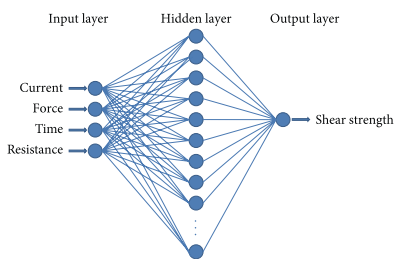
\includegraphics{./Bilder/The ANN structure for shear strength prediction.png}
\caption{The ANN structure for shear strength prediction}\label{fgg:ANN}
\end{figure}
Durch die Berechnung einer zuverlässigen Schätzung der Scherfestigkeit können Parametereinstellungen eine hohe Schweißqualität erzielen und reduziert sowohl die Zeit als auch den Probentest.
\newpage

\section{On-line Quality Estimation in Resistance Spot Welding\cite{Li.2000}}
Zwei Arten von Feature: die eine ist steuerbare Prozesseingangsvariablen und die andre ist Online-Signale (Elektroden Kraft, Verschiebung, dynamischer Widerstand)

Aufgrund der gekoppelten elektrisch-thermisch-mechanischen Natur weist RSW eine große Schwäche auf, d.H. es ist schwierig immer eine gut Qualität kontinuierlich zu bleiben. Die Qualität einer Schweißnaht wird im Allgemeinen durch Linsedurchmesser charakterisiert, der durch zerstörende Prüfung bestimmt wird.

In diesem Artikel wird eine Online-Methode zur Schätzung der Linsedurchmsser vorgestellt, die auf neuronalen Netzen und einer systematischen Merkmalsauswahl basiert. Es hat sich unter einer Vielzahl von Schweißbedingungen als erfolgreich erwiesen.

Das Linsewachstum ist abhängig von Elektroden Kraft und Verschiebung und dynamische Widerstand. Von jeder Kurve(Elektroden Kraft, Verschiebung, dynamischer Widerstand) können 24 Punkte gekriegt werden und wieder addieren 3 Variabel, Root Mean Square Strom, Vorkraft und Schweißzeit insgesamt 27 Feature.

In den 27 Feature können sie untereinander korreliert sein und daher können unnötige Informationen existieren. Um die Korrelation zu beseitigen, wurde eine PCA (Principal component  analysis) verwendet, d.h die Dimension kann reduziert basierend auf Varianzverhältnis werden.\\
\\
\textbf{Schweißparameter: }75 KVA Einphasen-Wechselstrom-Sockel Schweißer\\
\\
\textbf{Material: }0,8 mm AKDQ Stahl\\
\\
\textbf{Elektrode: }6,4 mm CuZr-Kegelstumpfelektroden\\
\\
\textbf{Qualitätsparameter: }Linsendurchmesser\\
\\
\textbf{Faktor: }

\begin{table}[H]
\caption{Faktor Tab. 2}
\begin{flushleft}
	\begin{tabular}{lc} 
		\toprule
 		\textbf{Faktor} & \textbf{Bedingungen} \\
		\midrule
		Elektrode Kraft(kN)& 3,0...4,0\\
		
		Strom(kA)& 6,9...13,4\\
		
		Zeit(Zyklen) & 3...36\\
		
		Kontaktdurchmesser(mm) & 6,4...7,2\\
		\bottomrule
	\end{tabular}
\end{flushleft}
\end{table}
Insgesamt 170 Proben werden unter verschiedenen Bedingungen gesammelt, davon 120 Randomsamples zum Training und 50 Samples zur Validierung.
Nach PAC (principal component analysis) wird Die Input Dimension auf 7 reduziert.
\begin{itemize}
\item Input:
\begin{itemize}
	\item 7 D
\end{itemize}
\item Hidden Layer1:
\begin{itemize}
	\item 14
\end{itemize}
\item Hidden Layer2:
\begin{itemize}
	\item 5
\end{itemize}
\item Output:
\begin{itemize}
	\item Linsendurchmesser
\end{itemize}
\end{itemize}
\begin{figure}[H]
\centering
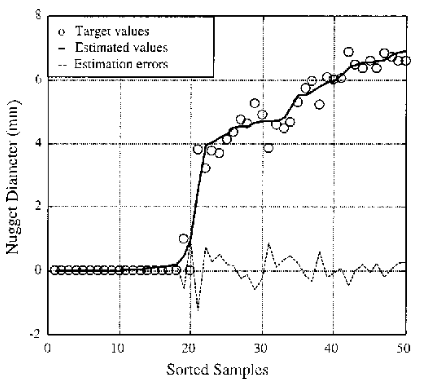
\includegraphics{./Bilder/Estimation results.png}
\caption{Estimation results}\label{fgg:Result}
\end{figure}




\newpage

\section{Artificial neural network-based resistance spot welding quality assessment syste\cite{ElOuafi.2011b}}
Neben Schweißparameter wie Schweißspannung, Strom, Zeit und Kraft gehören Elektrodenverschiebung, Elektroden Kraft, Temperaturschwankung, Schallemission, Ultraschallprüfung und dynamischer Widerstand ebenfalls zu wichtigen Qualitätsindikatoren in RSW. In diesen Indikatoren existieren dynamischer Widerstand und Qualitätsindikatoren deutlich Beziehung. \autoref{fig:DR} zeigt eine starke Korrelation zwischen den verschiedenen Entwicklungsphasen des RSW und der Form der DR Kurve.
Deswegen möchte der Autor die Feature durch Kombination zwischen Schweißparameter und DR Kurve in ANN benutzen 
\begin{figure}[H]
\centering
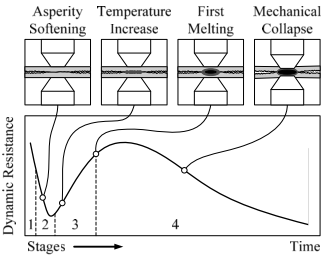
\includegraphics{./Bilder/Theoretical dynamic resistance curve and nugget formation stages.png}
\caption{Theoretical dynamic resistance curve and nugget formation stages}\label{fig:DR}
\end{figure}
\noindent
\textbf{Schweißmaschine: }tragbares Mittelfrequenz-DC-Schweißgerät\\
\\
\textbf{Material: }verzinkte kohlenstoffarme Stahlbleche\\
\\
\textbf{Elektrode: }wassergekühlte 45°-Kegelstumpf-RWMA-C2-Elektrode (CuCrZr) mit 8 mm Flächendurchmesser. Um Verschleiß und Zinkablagerungen zu minimieren, sollten die Elektroden durch Auswahl der geeigneten Elektrodenform und durch Verwendung von Wasserkühlung und Steuerung der Schweißgeschwindigkeit so kühl wie möglich gehalten werden.\\
\\
\textbf{Qualitätsparameter: }Elektrodeneindrucktiefe $e_{u}$, Linsendurchmesser $d_{n}$, Linseneindringtiefe $p$. Das resultierende Nugget wurde unter Verwendung eines metallografischen Standardverfahrens hergestellt und gemessen.\\
\begin{figure}[H]
\centering
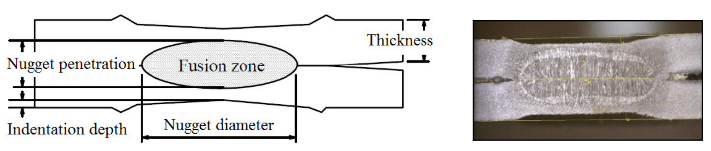
\includegraphics[scale = 0.8]{./Bilder/RSW quality indicators.png}
\caption{RSW quality indicators}\label{fig:RSW_QI}
\end{figure}
\noindent
\textbf{Faktor: }
\begin{table}[H]
\caption{Faktor Tab. 3}
\begin{flushleft}
	\begin{tabular}{lcc} 
		\toprule
 		\textbf{Faktor} & \textbf{Training sets} & \textbf{Validation sets}\\
		\midrule
		ST: Blechdicke(mm) & 0,95...1,85 & 0,95...1,85\\

		WC: Schweißstrom(A) & 6,25...9,50 & 6,25...9,50\\

		EF: Elektrodenkraft (N) & 184...400 & 184...400\\

		WT: Schweißzeit (s) & 300...500 & 300...500\\
		\bottomrule
	\end{tabular}
\end{flushleft}
\end{table}
wenn alle Parametereinstellung benutzt  und Wiederholung der Versuche zur Reduzierung des experimentellen Fehlers gemacht wird, kann max. insgesamt $3^4\times2 =162$ Versuche gebraucht werden. Offensichtlich wird so viel Versuche durchzuführen zu viel Zeit in Anspruch nehmen. Die Anzahl der Versuche wurde mit zwei OAs (L27 und L9) auf 36 reduziert.\\
\\
\textbf{Experiment Ergebnisse Analyse: }
\begin{figure}[H]
\centering
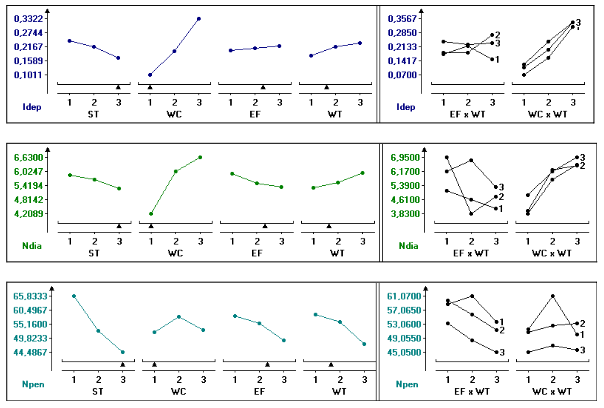
\includegraphics{./Bilder/Effect of Wpar and process conditions on the RSW quality indicators.png}
\caption{Effect of Wpar and process conditions on the RSW quality indicators}\label{fgg:AONVA1}
\end{figure}
\begin{figure}[H]
\centering
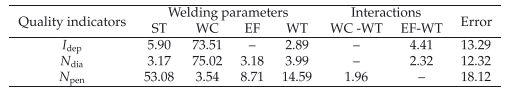
\includegraphics{./Bilder/Percent contributions of Wpar in the variation of the quality indicators.png}
\caption{Percent contributions of Wpar in the variation of the quality indicators}\label{fgg:AONVA2}
\end{figure}
Diese Ergebnisse zeigen, dass der Fehlerbeitrag relativ hoch ist. Dies bedeutet, dass wichtige Faktoren, die die RSW-Qualität beeinflussen, nicht in die Experimente einbezogen wurden. Dementsprechend kann davon ausgegangen werden, dass die Qualitätsindikatoren nicht nur mit ST, WC und WT gesteuert werden können.\\
\\
\textbf{ANN: }\\
Neue Qualitätsindikatoren ST WC EF WT und DR (mit mindestens 6 gleichmäßig verteilten Punkten). 
\begin{itemize}
\item Input:
\begin{itemize}
	\item n
\end{itemize}
\item Hidden Layer1:
\begin{itemize}
	\item 2n+1
\end{itemize}
\item Output:
\begin{itemize}
	\item Elektrodeneindrucktiefe $e_{u}$
	\item Linsendurchmesser $d_{n}$ 
	\item Linseneindringtiefe $p$
\end{itemize}
\end{itemize}
Für Feature Selection könnte OA L8 verwendet werden.
\begin{figure}[H]
\centering
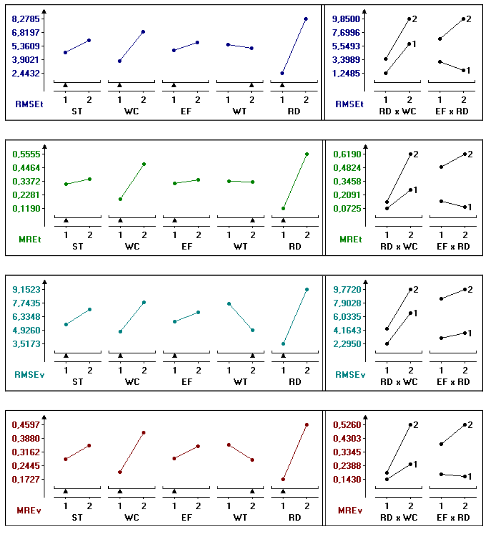
\includegraphics{./Bilder/Average effects of each variable in increasing or decreasing themodeling performance criteria.png}
\caption{Average effects of each variable in increasing or decreasing themodeling performance criteria}\label{fgg:AONVA3}
\end{figure}
\begin{figure}[H]
\centering
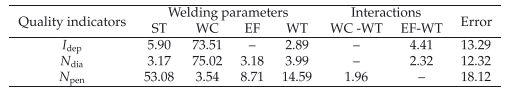
\includegraphics{./Bilder/Percent contributions of Wpar in the variation of the quality indicators.png}
\caption{Percent contributions of Wpar in the variation of the quality indicators}\label{fgg:AONVA4}
\end{figure}
\begin{figure}[H]
\centering
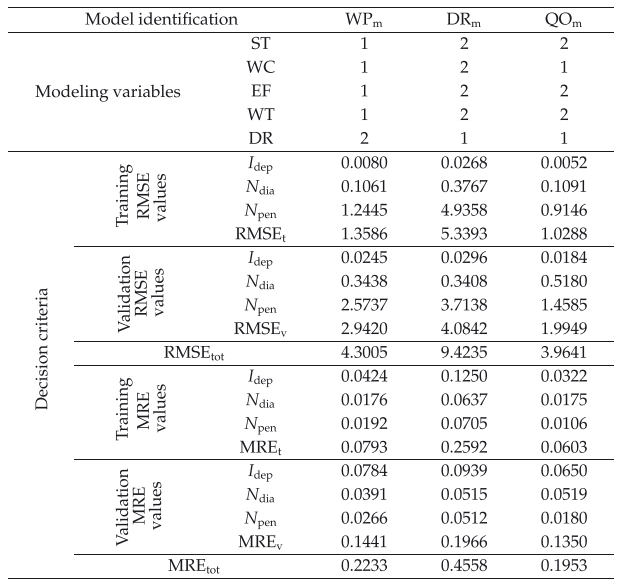
\includegraphics{./Bilder/Modeling evaluation results.png}
\caption{Modeling evaluation results}\label{fgg:evaluation results}
\end{figure}

Ein quasi optimales Modell entwickelt, das \textbf{Schweißparameter} und typische Eigenschaften des \textbf{dynamischen Widerstands} kombiniert.
\begin{figure}[H]
\centering
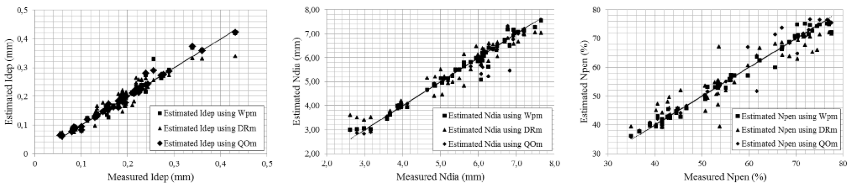
\includegraphics[scale = 0.7]{./Bilder/Model evaluation using measured and estimated quality indicators.png}
\caption{Model evaluation using measured and estimated quality indicators}\label{fgg:Model evaluation}
\end{figure}

\newpage
\section{Online qualitative nugget classification by using a linear vector quantization neural network for resistance spot welding\cite{ElBanna.2008}}
In diesem Artikel wird ein algorithmisches Framework vorgeschlagen, das auf einem neuronalen Netzwerk mit linear vector quantization (LVQ) basiert und die Klassifizierung von Linsequalität  basierend auf einer kleinen Anzahl dynamischer Widerstandsmuster für Kalt-, Normal- und Spritzer schätzt, die während des Stabilisierungsprozesses gesammelt werden.

Die Klassifizierung der Linse-Qualität mithilfe eines LVQ-Netzwerks wurde auf zwei Arten von Controllern getestet: MFDC mit konst. Stromregler and AC mit konst. Wärmeregler.

Um die Dimension des Eingabedatenvektors zu verringern, werden verschiedene Punkt aus dem dynamischen Widerstandsprofil extrahiert und unter Verwendung der Leistung der Testkriterien verglichen.\\
\\
\textbf{Schweißmaschine: }MFDC mit Konstantstromregler, AC mit konstantem Wärmeregler\\
\\
\textbf{Material: }2,00 mm Feuerverzinkter HSLA-Stahl mit 0,85 mm Galvanisch verzinkter HSLA-Stahl\\
\\
\textbf{Elektrode: }HWPAL25 mit einem Flächendurchmesser von 6,4 mm\\
\\
\textbf{Faktor: }\\
\begin{table}[H]
\caption{Faktor Tab. 4}
\begin{flushleft}
	\begin{tabular}{lcc} 
		\toprule
 		\textbf{Faktor} & \textbf{MFDC(Konstantstromregler)} & \textbf{AC(Konstantwärmeregler)}\\
		\midrule
		Schweißstrom(kA) & 11,5 mit 1 A Anstieg pro Schweißung. & 11,3\\

		Elektrodenkraft(lb) & 680 & 680\\

		Schweißzeit & 233 ms & 16 Zyklen\\
		\bottomrule
	\end{tabular}
\end{flushleft}
\end{table}

Elf Batches mit jeweils 300 Schweißnähten (insgesamt 3,300 Schweißnähte ohne Ankerschweißpunkte) wurden mit 10 Elektroden durchgeführt, die nach jeden Batches bearbeitet wurden.Im Fall des MFDC Tests wurde jedes Batche 50 Samples ausgewählt. Deswegen wurde insgesamt 550 Linsedurchmesser gemessen. Davon haben 411 mit guter Qualität, 22 mit schlecht Qualität und 117 mit Spritzer.

Im Fall des AC Tests wurde 720 Samples ausgewählt. Davon 509 mit guter Qualität und 211 mit Spritzer

In allen Tests basiert die Klassifizierung der  Linse-Qualität auf dem Widerstandsprofil
\begin{figure}[H]
\centering
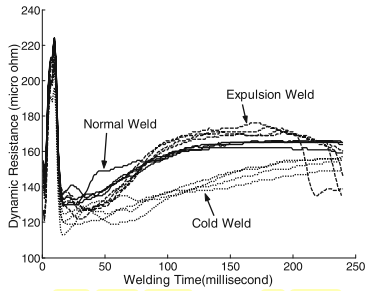
\includegraphics{./Bilder/Sample dynamic resistance profiles for cold, expulsion, and normal welds for a CCC using MFDC.png}
\caption{Sample dynamic resistance profiles for cold, expulsion, and normal welds for a CCC using MFDC}\label{fgg:MFDC_DR}
\end{figure}
\begin{figure}[H]
\centering
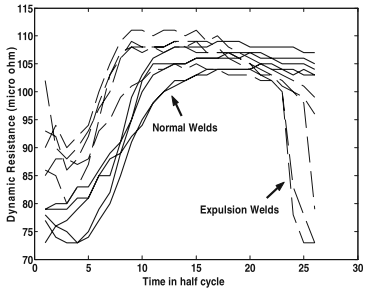
\includegraphics{./Bilder/Sample dynamic resistance profile for cold, expulsion and normal welds for an AC constant heat controller.png}
\caption{Sample dynamic resistance profile for cold, expulsion and normal welds for an AC constant heat controller}\label{fgg:AC_DR}
\end{figure}


Das LVQ-Modell wurde an 3, 6 und 5 Samples des sekundären Widerstandsvektors für Kalt-, Normal- bzw. Spritzer-Schweiß trainiert.
 
\textbf{LVQ: }
\begin{itemize}
\item MFDC Konstantstromregler
\begin{itemize}
\item Input:
\begin{itemize}
	\item 167 Dimension gleich der Anzahl der Millisekunden-Samples in einem Schweißen ohne die ersten 67 ms
\end{itemize}
\item Hidden Layer:
\begin{itemize}
	\item 12
\end{itemize}
\item Output:
\begin{itemize}
	\item schlecht 
	\item gut 
	\item Spritzer
\end{itemize}
\end{itemize}
\item AC  Konstantwärmeregler
\begin{itemize}
\item Input:
\begin{itemize}
	\item 24 Dimension gleich der Anzahl der Halbzyklen in einem Schweißen nach der Vorheiz- und Abkühlphase
\end{itemize}
\item Hidden Layer:
\begin{itemize}
	\item 12
\end{itemize}
\item Output:
\begin{itemize}
	\item schlecht 
	\item gut 
	\item Spritzer
\end{itemize}
\end{itemize}
\end{itemize}

Um die Dimension des Eingangs zu verringern, wurde der tatsächliche Widerstandsvektor durch eine Reihe repräsentativer Merkmale ersetzt.

\begin{itemize}
\item $R_{max}$
\item $R_{min}$
\item $\bar R$
\item $SD$ des Eingangswiderstands
\item $\Delta R$
\item $RMS$
\item Steigungswert der ersten Region ($S1$) des Eingangswiderstands
\item Steigungswert der zweiten Region ($S2$) des Eingangswiderstands
\item Steigungswert der dritten Region ($S3$) des Eingangswiderstands
\item Steigungswert der vierten Region ($S4$) des Eingangswiderstands
\item Binned $RMS$ des Eingangswiderstands; Der Eingangswiderstand ist in fünf Bins unterteilt und die $RMS$ werden für jeden Bin berechnet
\end{itemize}

Die Ergebnisse aus der Anwendung des LVQ neuronales Netz trainiert, indem sie die sehr begrenzte Daten während des Stabilisierungsprozesses gesammelt verwenden, sind sehr vielversprechend und werden im Detail berichtet.\\
Darüber hinaus berichten wir viel versprechende Ergebnisse sehr, wenn ein reduzierter Feature für die Einstufung verwendet wird, anstatt das gesamte dynamisches Widerstandsprofil.
\newpage

\section{Identification in Resistance Spot Welding by Electrode Force Sensing Based on Wavelet Decomposition with Multi-Indexes and BP Neural Networks\cite{Chen.2019}}
Die Spritzeridentifikation hat für die Bewertung und Kontrolle der Schweißqualität beim RSW größe Bedeutung. Um die Identifikationsgenauigkeit zu verbessern, wurden neuartige neuronale Netze für Wavelet decomposition und Back Propagation (BP) mit der Peak-Peak-Amplitude und dem Kurtosis-Index vorgeschlagen um den Spritzer von Elektrodenkraft-Erfassungssignalen zu identifizieren.

Das Elektrodenkraftsignal ist ein typisches instationäres Signal, dessen verteilte Parameter sich mit der Zeit ändern. Daher konnte weder die Zeitbereichsanalyse noch die Frequenzbereichsanalyse das Signal genau ausdrücken. Die Wavelet-decomposition ist eine Art stabiles und schnelles Zeit-Frequenz-Signalanalyseverfahren.\\
\begin{figure}[H]
\centering
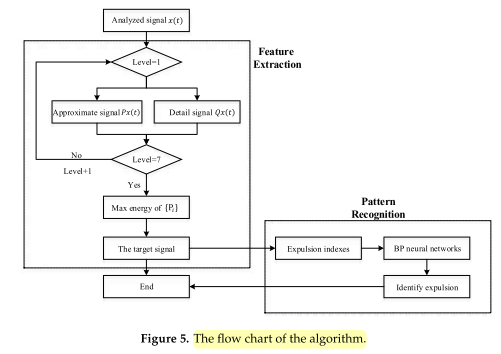
\includegraphics{./Bilder/The flow chart of the algorithm.png}
\caption{The flow chart of the algorithm}\label{fgg:Wvelets}
\end{figure}

\textbf{Signal Processing: }
Der Prozess führte eine mehrstufige eindimensionale Wavelet-Analyse unter Verwendung spezifischer Wavelet-Zerlegungsfilter durch, einschließlich des Tiefpassfilters und des Hochpassfilters.
\begin{figure}[H]
\centering
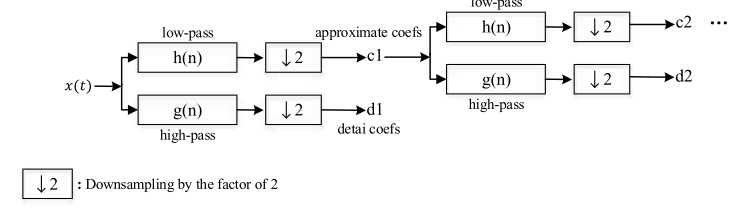
\includegraphics[scale = 0.8]{./Bilder/Flow chart of the coefs.png}
\caption{Flow chart of the coefs}\label{fgg:Wavelets}
\end{figure}
Schließlich wurde die Energie jedes Detailsignals Qx (t) berechnet und das höchste als Zielsignal ausgewählt. Die Peak-Peak-Amplitude und dem Kurtosis-Index des Zielsignals wurden als Eingabeparameter des BP Neur berechnet.
Folgende sind 3 typische Kraftsignals,daher könnte die Anschlag-Feature als Hauptspritzerfmerkmal bei der Unterscheidung des Spritzer verwendet werden.
\begin{figure}[H]
\centering
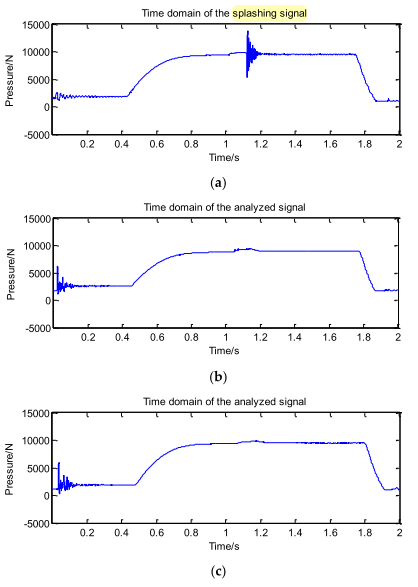
\includegraphics[scale = 0.8]{./Bilder/The time domain of the electrode force signal.png}
\caption{The time domain of the electrode force signal}\label{fgg:Kraftsg}
\end{figure}
Durch Wavelet decomposition wurde die Signals auf jeden Layer bokommen:

\begin{figure}[H]
\centering
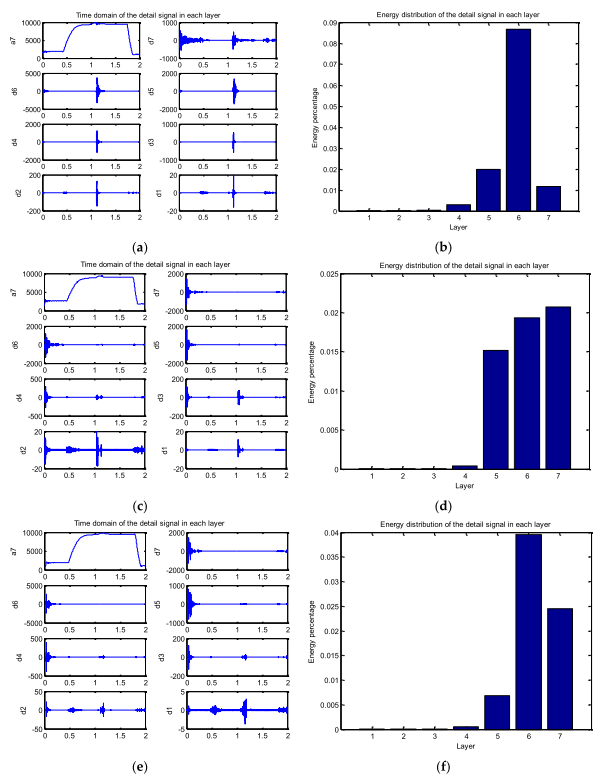
\includegraphics[scale = 0.8]{./Bilder/expulsion signal.png}
\caption{expulsion signal}\label{fgg:Wavelets}
\end{figure}
In dieser Arbeit wurde der Energieverteilung des Signals in jeder Schicht berechnet und das höchste als Zielsignal ausgewählt.
\begin{figure}[H]
\centering
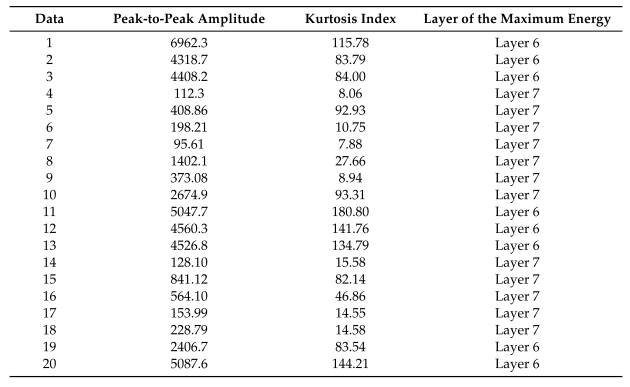
\includegraphics[scale = 0.8]{./Bilder/The characteristic indexes of the target signal.png}
\caption{The characteristic indexes of the target signal}\label{fgg:Wavelets}
\end{figure}
\begin{figure}[H]
\centering
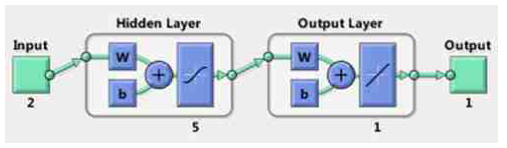
\includegraphics[scale = 0.8]{./Bilder/The structure of the BP neural network.png}
\caption{The structure of the BP neural network}\label{fgg:Wavelets}
\end{figure}
\begin{itemize}
\item Input:
\begin{itemize}
	\item Peak-Peak-Amplitude 
	\item Kurtosis-Index
\end{itemize}
\item Hidden Layer:
\begin{itemize}
	\item 5
\end{itemize}
\item Output:
\begin{itemize}
	\item 1 oder -1 (1: Spritzer, -1: ohne Spritzer)
\end{itemize}
\end{itemize}
\newpage
\section{Performances of regression model and artificial neural network in monitoring welding quality based on power signal\cite{Zhao.2020}}
In dieser Studie wurde eine Untersuchung durchgeführt, um die Leistung des Regressionsmodells und des künstlichen neuronalen Netzwerks bei der Vorhersage des Linsendurchmesser von RSW durch Überwachung der dynamischen Leistungssignatur zu vergleichen.

Ein Echtzeit-Erfassungssystem vorgestellt, nach dem der Schweißstrom und die Schweißspannung im Sekundärkreis erhalten wurden. Das Leistungssignal wurde erfasst und analysiert, um die Schweißqualitäten zu charakterisieren. Die Schweißqualitäten können als schlechte , gute Spritzer-Schweißnähte klassifiziert werden. Die Feature mit physikalischen Bedeutungen wurden aus dem Leistungssignal extrahiert, um die Variationen im Signal zu identifizieren, und sie wurden dann als Eingaben des künstlichen neuronalen Netzwerks und des Regressionsmodells benutzt. Die Vorhersagegenauigkeit der Modelle wurde ebenfalls diskutiert.


\newpage
\printbibliography[heading=bibintoc]\label{sec:bibliography}%



\end{document}
